\chapter{Conception}


% ----------------------------------------------------------------------------- Cas d'utilisations

\section{Description d\'etaill\'ee des cas d’ utilisation}

\subsection{Charger un plan}
\begin{description}
    \item[Contexte :] le superviseur veut visualiser le plan d'une zone de la ville
    \item[Acteur principal :] Superviseur
    \item[Precondition :] -
    \item[Postconditions :] Le plan doit \^etre affich\'e
    \item[Scenario principal :] ~
    \begin{enumerate}
        \item Le superviseur demande le chargement d'un plan pour une zone de la ville
        \item Le syst\`eme demande au SGBD si la zone existe bien, ainsi que les donn\'ees correspondantes
        \begin{enumerate}
            \item La zone n'existe pas :
            \begin{enumerate}
                \item Le syst\`eme renvoie une erreur, le CdU reprend \`a l'\'etape 1, le cas d'utilisation se termine par un \'echec.
            \end{enumerate}
            \item Erreur syntaxique, le cas d'utilisation se termine par un \'echec.
            \item Erreur s\'emantique, le cas d'utilisation se termine par un \'echec.
        \end{enumerate}
        \item Le syst\'eme affiche le plan \`a l'\'ecran, le cas d'utilisation se termine par un succ\`es.
    \end{enumerate}
\end{description}
\pagebreak

\subsection{Charger une demande de livraison}
\begin{description}
    \item[Contexte :] Le superviseur veut charger une demande de livraison, c'est-\`a-dire un ensemble de points \`a livrer avec, pour chaque point, sa
    plage horaire
    \item[Acteur principal :] Superviseur
    \item[Precondition :] Le plan doit \^etre charg\'e
    \item[Postconditions :] Les points doivent \^etre affich\'es sur le plan
    \item[Scenario principal :] ~
    \begin{enumerate}
        \item Le superviseur s\'electionne une demande de livraison
        \item Le syst\`eme demande au SGBD si la demande de livraison existe bien, ainsi que les donn\'ees correspondantes
        \begin{enumerate}
            \item La demande de livraison n'existe pas :
            \begin{enumerate}
                \item Le syst\'eme renvoie une erreur, le CdU reprend \`a l'\'etape 1, le cas d'utilisation se termine par un \'echec.
            \end{enumerate}
            \item Erreur syntaxique, le cas d'utilisation se termine par un \'echec.
            \item Erreur s\'emantique, le cas d'utilisation se termine par un \'echec.
        \end{enumerate}
        \item Le syst\`eme affiche les points de livraison sur le plan, le cas d'utilisation se termine par un succ\`es.
    \end{enumerate}
\end{description}

\subsection{Calculer une tourn\'ee}
\begin{description}
    \item[Contexte :] Le superviseur veut calculer une tourn\'ee pour la derni\`ere demande de livraisons charg\'ee
    \item[Acteur principal :] Superviseur
    \item[Precondition :] Une tourn\'ee doit \^etre selectionn\'ee, les demandes de livraisons doivent \^etre charg\'ees
    \item[Postconditions :] -
    \item[Scenario principal :] ~
    \begin{enumerate}
        \item Le superviseur clique sur "calculer tourn\'ee" pour la demande de livraison
        \item Le syst\`eme calcule la tourn\'ee et l'envoie au SGBD
        \begin{enumerate}
            \item Il n'est pas possible de tout faire dans les temps, le syst\`eme notifie l'utilisateur qu'il y aura forc\'ement des retards, le cas d'utilisation se termine par un succ\`es.
            \item Une livraison n'est pas accessible, le cas d'utilisation se termine par un \'echec.
        \end{enumerate}
        \item Le syst\`eme affiche la tourn\'ee sur le plan, le cas d'utilisation se termine par un succ\`es.
    \end{enumerate}
\end{description}
\pagebreak

\subsection{Visualiser une tourn\'ee}
\begin{description}
    \item[Contexte :] Le superviseur veut visualiser une tourn\'ee sur un plan avec les diff\'erents \'etats des livraisons (fait, \`a l'heure, en retard, etc.). Possibilit\'e de visualiser les details de la tourn\'ee.
    \item[Acteur principal :] Superviseur
    \item[Precondition :] La tourn\'ee existe et est dans une liste de tourn\'ees disponibles
    \item[Postconditions :] La tourn\'ee existe, est dans une liste de tourn\'ees disponibles, est selectionn\'ee et est affich\'ee
    \item[Scenario principal :] ~
    \begin{enumerate}
        \item Le superviseur clique sur la tourn\'ee dans la liste
        \item La tourn\'ee s'affiche dans la zone pr\'evue \`a cet effet
    \end{enumerate}
    \item[Extension :] ~
    \begin{enumerate}
        \item Le superviseur clique sur "d\'etail"
        \begin{enumerate}
            \item Les informations compl\'ementaires s'affichent dans la zone pr\'evue \`a cet effet, le cas d'utilisation se termine par un succ\`es.
            \item Les informations par d\'efaut s'affichent si la tourn\'ee est vide, le cas d'utilisation se termine par un succ\`es.
        \end{enumerate}
    \end{enumerate}
\end{description}

\subsection{G\'en\'erer d'une feuille de route}
\begin{description}
    \item[Contexte :] Le superviseur veut g\'en\'erer une feuille de route d'un livreur contenant les itin\'eraires de chaque livraison
    \item[Acteur principal :] Superviseur
    \item[Precondition :] La tourn\'ee du livreur est pr\^ete.
    \item[Postconditions :] La feuille de route a \'et\'e g\'en\'er\'ee et la version papier imprim\'ee
    \item[Scenario principal :] ~
    \begin{enumerate}
        \item Le superviseur clique sur "g\'en\'erer feuille de route"
        \item La feuille de route est g\'en\'er\'ee et sauvegard\'ee, le cas d'utilisation se termine par un succ\`es.
        \begin{enumerate}
            \item Pas de livraison pour la tourn\'ee
            \item Probl\`eme avec l'ordinateur pendant la sauvegarde
            \item Le fichier existe d\'ej\`a dans les sauvegardes
            \begin{enumerate}
                \item Ecraser l'ancien, le cas d'utilisation se termine par un succ\`es.
                \item Annuler le nouveau, le cas d'utilisation se termine par un \'echec.
                \item Renomer l'un des deux, le cas d'utilisation se termine par un succ\`es.
            \end{enumerate}
        \end{enumerate}
    \end{enumerate}
\end{description}
\pagebreak

\subsection{Modifier une tourn\'ee en temps r\'eel}
\begin{description}
    \item[Contexte :] Le superviseur veut modifier une tourn\'ee le jour m\^eme en ajoutant ou retirant une livraison. Il doit \^etre possible d'annuler la derni\`ere action, mais aussi de la refaire.
    \item[Acteur principal :] Superviseur
    \item[Preconditions :] ~
    \begin{description}
        \item[G\'en\'erale :] Il y a une tourn\'ee s\'electionn\'ee, il est possible de communiquer avec le livreur
        \item[Pour ajouter :] Il y a au moins un noeud libre sur le plan
        \item[Pour enlever :] Il y a au moins une livraison dans la tourn\'ee
    \end{description}
    \item[Postconditions :] ~
    \begin{description}
        \item[G\'en\'erale :] La tourn\'ee s\'electionn\'ee est modifi\'ee et les changements ont \'et\'e envoy\'es au livreur
        \item[Pour ajouter :] La livraison est ajout\'ee \`a la tourn\'ee \`a la bonne place
        \item[Pour enlever :] La livraison est enlev\'ee de la tourn\'ee qui est automatiquement recalcul\'ee
    \end{description}
    \item[Scenario principal :] ~
    \begin{description}
        \item[Ajouter] ~
        \begin{enumerate}
            \item Le superviseur selectionne un noeud disponible
            \item Le superviseur clique sur "ajouter" et remplit le forumlaire d'ajout (plage horaire, client, etc.)
            \item Le superviseur clique sur "annuler" pendant qu'il remplit le formulaire
            \begin{enumerate}
                \item L'ajout est annul\'e et le superviseur perd ce qu'il avait pr\'e-rempli, le cas d'utilisation se termine par un \'echec.
            \end{enumerate}
            \item Le supervieur clique sur "ok"
            \item La livraison est ajout\'ee et la tourn\'ee recalcul\'ee
            \item L'ajout est envoy\'e au livreur, le cas d'utilisation se termine par un succ\`es.
            \begin{enumerate}
                \item La connexion au livreur \'echoue, le cas d'utilisation se termine par un \'echec.
            \end{enumerate}
        \end{enumerate}
        \item[Enlever] ~
        \begin{enumerate}
            \item Le superviseur selectionne une livraison sur la tourn\'ee
            \item Le superviseur clique sur "enlever"
            \item La livraison est enlev\'ee et la tourn\'ee recalcul\'ee
            \begin{enumerate}
                \item La livraison est enlev\'ee et la tourn\'ee est vide, le syst\'eme continue \`a l'\'etape enlever:4
            \end{enumerate}
            \item La suppression est envoy\'ee au livreur, le cas d'utilisation se termine par un succ\`es.
            \begin{enumerate}
                \item La connexion au livreur \'echoue, le cas d'utilisation se termine par un \'echec.
            \end{enumerate}
        \end{enumerate}
    \end{description}
\end{description}
\pagebreak

\subsection{Pr\'e-modifier une tourn\'ee}
\begin{description}
    \item[Contexte :] Le superviseur veut modifier une tourn\'ee la veille en ajoutant ou retirant une livraison. Il doit \^etre possible d'annuler la derni\`ere action, mais aussi de la refaire.
    \item[Acteur principal :] Superviseur
    \item[Preconditions :] ~
    \begin{description}
        \item[G\'en\'erale :] Il y a une tourn\'ee s\'electionn\'ee, il est possible de communiquer avec le livreur
        \item[Pour ajouter :] Il y a au moins un noeud libre sur le plan
        \item[Pour enlever :] Il y a au moins une livraison dans la tourn\'ee
    \end{description}
    \item[Postconditions :] ~
    \begin{description}
        \item[G\'en\'erale :] La tourn\'ee s\'electionn\'ee est modifi\'ee
        \item[Pour ajouter :] La livraison est ajout\'ee \`a la tourn\'ee \`a la bonne place
        \item[Pour enlever :] La livraison est enlev\'ee de la tourn\'ee qui est automatiquement recalcul\'ee
    \end{description}
    \item[Scenario principal :] ~
    \begin{description}
        \item[Ajouter] ~
        \begin{enumerate}
            \item Le superviseur selectionne un noeud disponible
            \item Le superviseur clique sur "ajouter" et remplit le forumlaire d'ajout (plage horaire, client). La plage horaire se decompose en deux champs chiffr\'es qui doivent \^etre coh\'erents avec la notion de plage horaire
            \item Le superviseur clique sur "annuler" pendant qu'il remplit le formulaire
            \begin{enumerate}
                \item L'ajout est annul\'e et le superviseur perd ce qu'il avait pr\'e-rempli, le cas d'utilisation se termine par un \'echec.
            \end{enumerate}
            \item Le supervieur clique sur "ok"
            \begin{enumerate}
                \item Une aberration est dans la livraison \`a ajouter, le syst\`eme signale une erreur, le cas d'utilisation se termine par un \'echec.
            \end{enumerate}
            \item La livraison est ajout\'ee et la tourn\'ee recalcul\'ee, le cas d'utilisation se termine par un succ\`es.
        \end{enumerate}
        \item[Enlever] ~
        \begin{enumerate}
            \item Le superviseur selectionne une livraison sur la tourn\'ee
            \item Le superviseur clique sur "enlever"
            \item La livraison est enlev\'ee et la tourn\'ee recalcul\'ee, le cas d'utilisation se termine par un succ\`es.
            \begin{enumerate}
                \item La livraison est enlev\'ee et la tourn\'ee est vide, le cas d'utilisation se termine par un succ\`es.
            \end{enumerate}
        \end{enumerate}
    \end{description}
\end{description}
\pagebreak


% ----------------------------------------------------------------------------- Diagrames-UML

\section{Diagrammes de packages et de classes}

\begin{figure}[h]
    \centering
    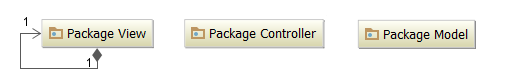
\includegraphics[width=80mm]{../diagrams/classes_packages/classes_packages/packages.png}
    \caption{Diagramme UML de package principale}
    \label{diagram:uml_global}
\end{figure}

\subsection{Mod\`ele (Model)}

\begin{figure}[h]
    \centering
    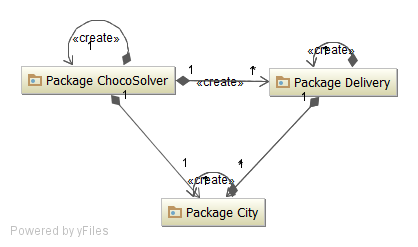
\includegraphics[width=80mm]{../diagrams/classes_packages/classes_packages/model/package_model.png}
    \caption{Diagramme UML du package Model}
    \label{diagram:uml_model}
\end{figure}
\pagebreak

\subsubsection{Mod\`ele Ville (Model.City)}

\begin{figure}[h]
    \centering
    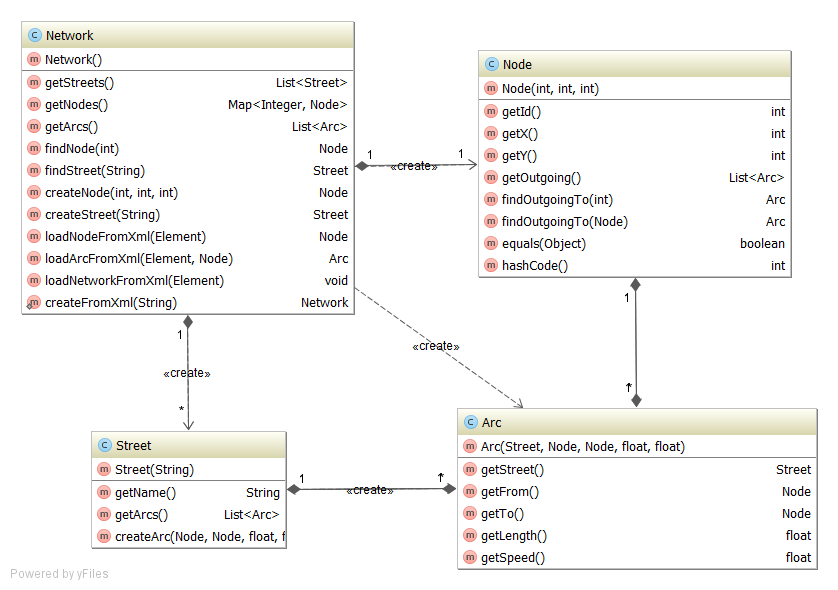
\includegraphics[width=160mm]{../diagrams/classes_packages/classes_packages/model/city.png}
    \caption{Diagramme UML du package Model.City}
    \label{diagram:uml_model_city}
\end{figure}
\pagebreak

\subsubsection{Mod\`ele Livraison (Model.Delivery)}

\begin{figure}[h]
    \centering
    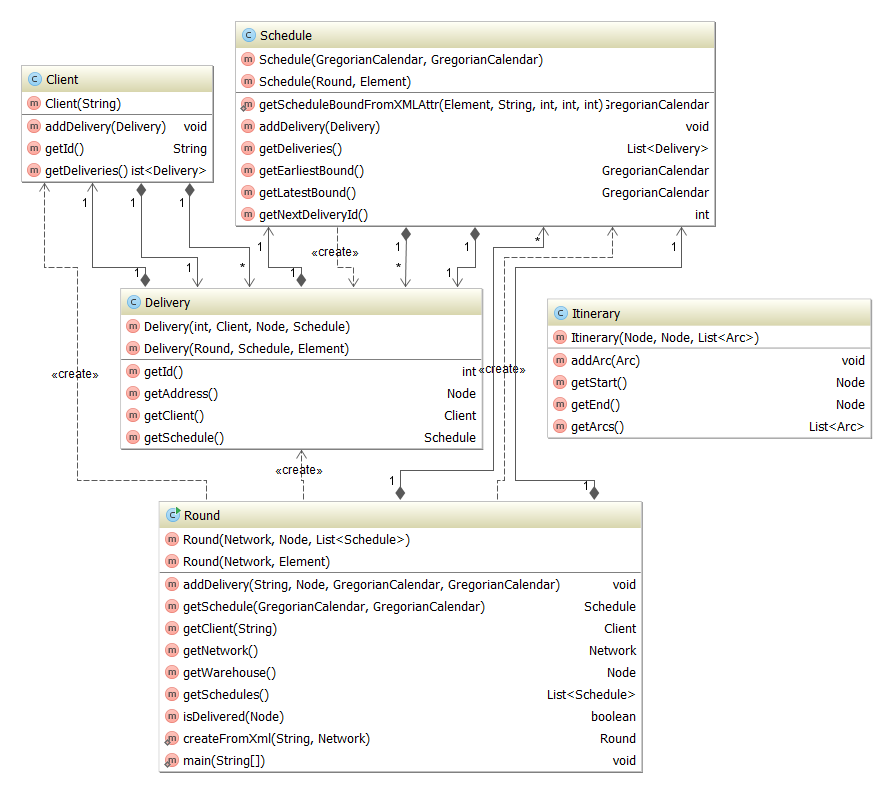
\includegraphics[width=160mm]{../diagrams/classes_packages/classes_packages/model/delivery.png}
    \caption{Diagramme UML du package Model.Delivery}
    \label{diagram:uml_model_delivery}
\end{figure}
\pagebreak

\begin{landscape}
\subsubsection{Mod\`ele Resolution Choco (Model.ChocoSolver)}

\begin{figure}[h]
    \centering
    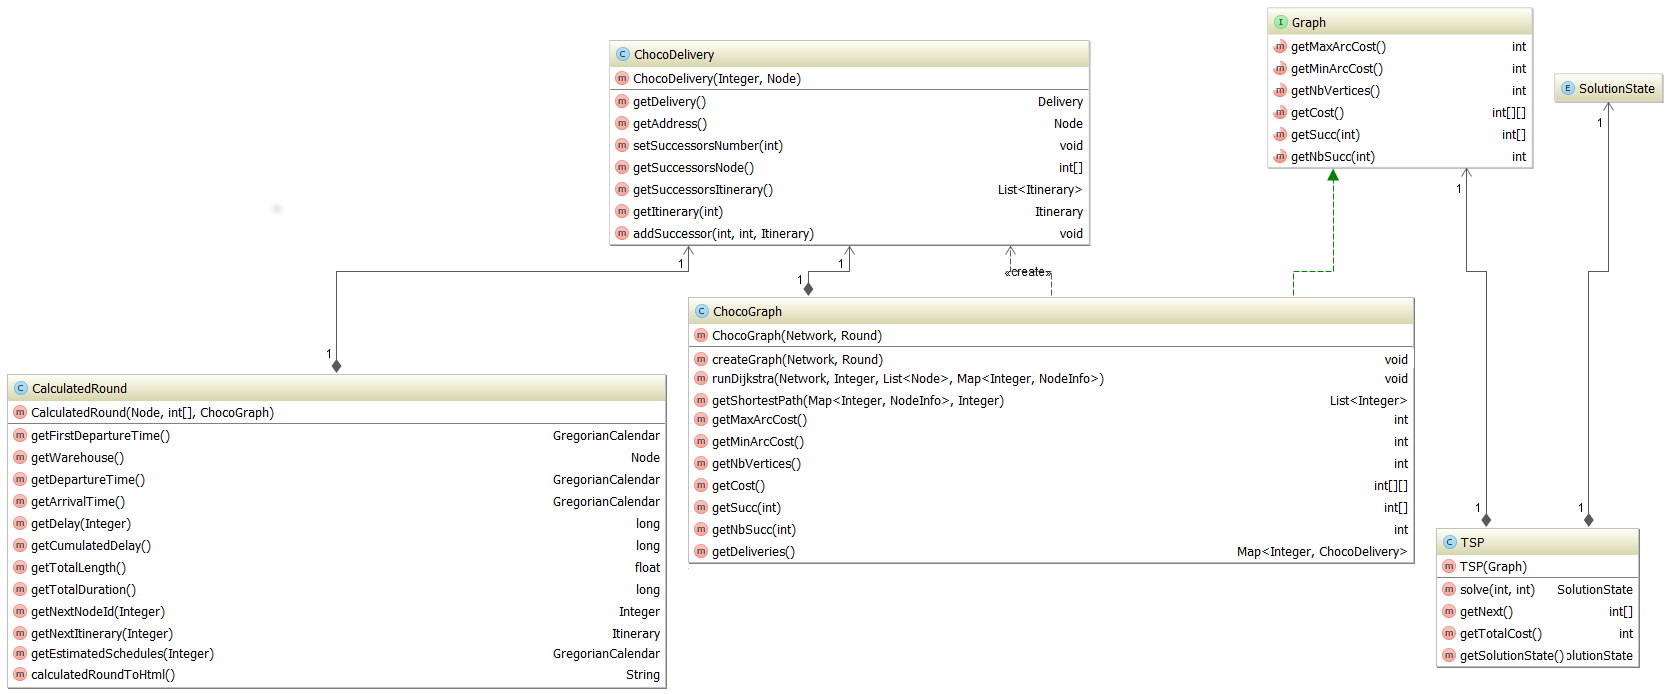
\includegraphics[width=240mm]{../diagrams/classes_packages/classes_packages/model/chocoSolver.png}
    \caption{Diagramme UML du package Model.ChocoSolver}
    \label{diagram:uml_model_choco}
\end{figure}
\end{landscape}
\pagebreak

\subsection{Vue (View)}

\begin{figure}[h]
    \centering
    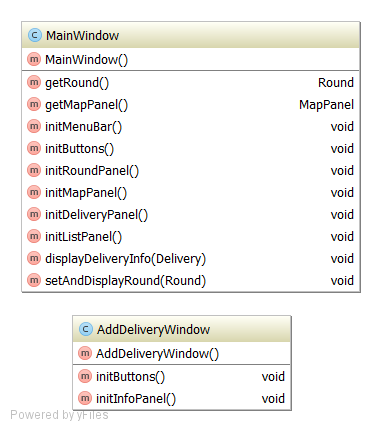
\includegraphics[width=80mm]{../diagrams/classes_packages/classes_packages/view/view.png}
    \caption{Diagramme UML du package View}
    \label{diagram:uml_view}
\end{figure}
\pagebreak

\subsubsection{Vue Carte (View.MapPanel)}

\begin{figure}[h]
    \centering
    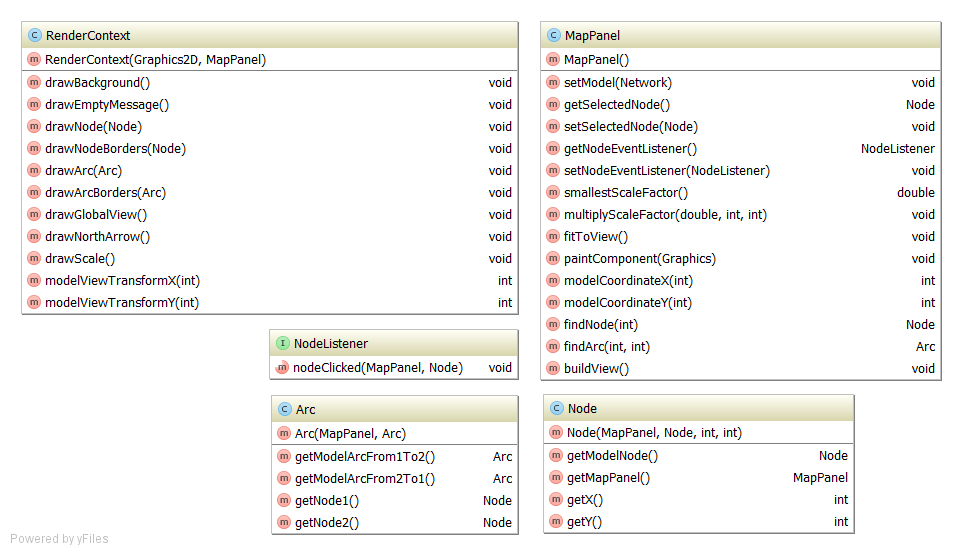
\includegraphics[width=160mm]{../diagrams/classes_packages/classes_packages/view/package_map.png}
    \caption{Diagramme UML du package View.MapPanel}
    \label{diagram:uml_view_map}
\end{figure}
\pagebreak

\subsection{Controlleur (Controller)}

\begin{figure}[h]
    \centering
    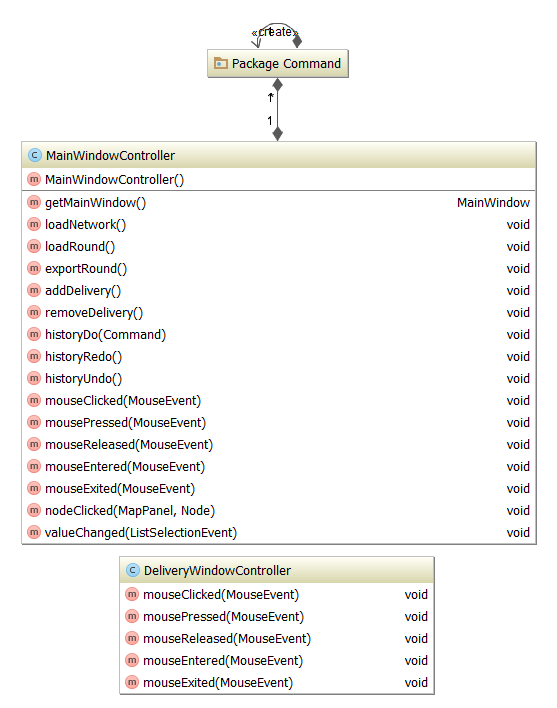
\includegraphics[width=80mm]{../diagrams/classes_packages/classes_packages/controller/controller.png}
    \caption{Diagramme UML du package Controller}
    \label{diagram:uml_controller}
\end{figure}
\pagebreak

\subsubsection{Commande (Controller.Command)}

\begin{figure}[h]
    \centering
    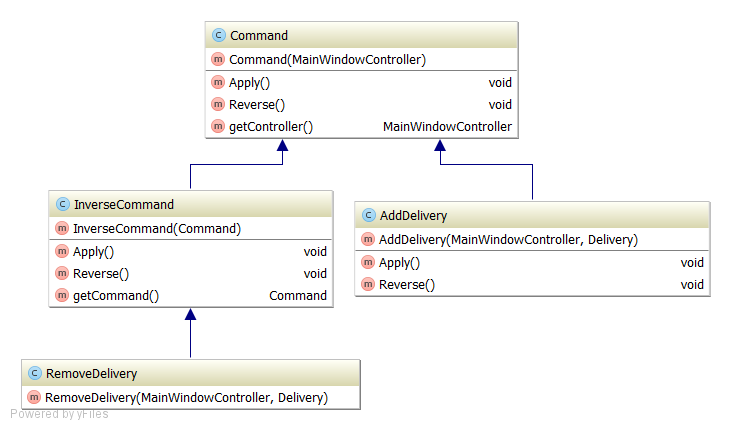
\includegraphics[width=160mm]{../diagrams/classes_packages/classes_packages/controller/package_command.png}
    \caption{Diagramme UML du package Controller.Command}
    \label{diagram:uml_controller_command}
\end{figure}

Ce package implemente le design pattern Commande afin de g\'erer le undo/redo pour l'ajout et
suppression d'une livraison dans la tourn\'ee.

On remarque alors que les classes AddDelivery et
RemoveDelivery ont un code pour les m\'ethodes Apply() et Reverse() semblable \`a la diff\'erence
qu'ils sont invers\'es (la fonction Apply() de RemoveDelivery est identique a Reverse() de
AddDelivery par exemple). Dans un but de factorisation de code pour l'ajout
et la suppression, nous avons donc choisi d'impl\'ementer la classe InverseCommand. Celle-ci est donc une
commande effectuant les op\'erations inverses d'une autre qu'on lui passe \`a l'instanciation.

Ainsi nous pouvons impl\'ementer RemoveDelivery en faisant simplement l'inverse de la commande
AddDelivery. Autrement dit, pour supprimer une livraison, il suffit de la "d\'esajouter".


% ----------------------------------------------------------------------------- Sequences

\begin{landscape}
    \section{Diagramme de s\'equences}

    \subsection{Chargement d'un tourn\'ee}

    \begin{figure}[h]
        \centering
        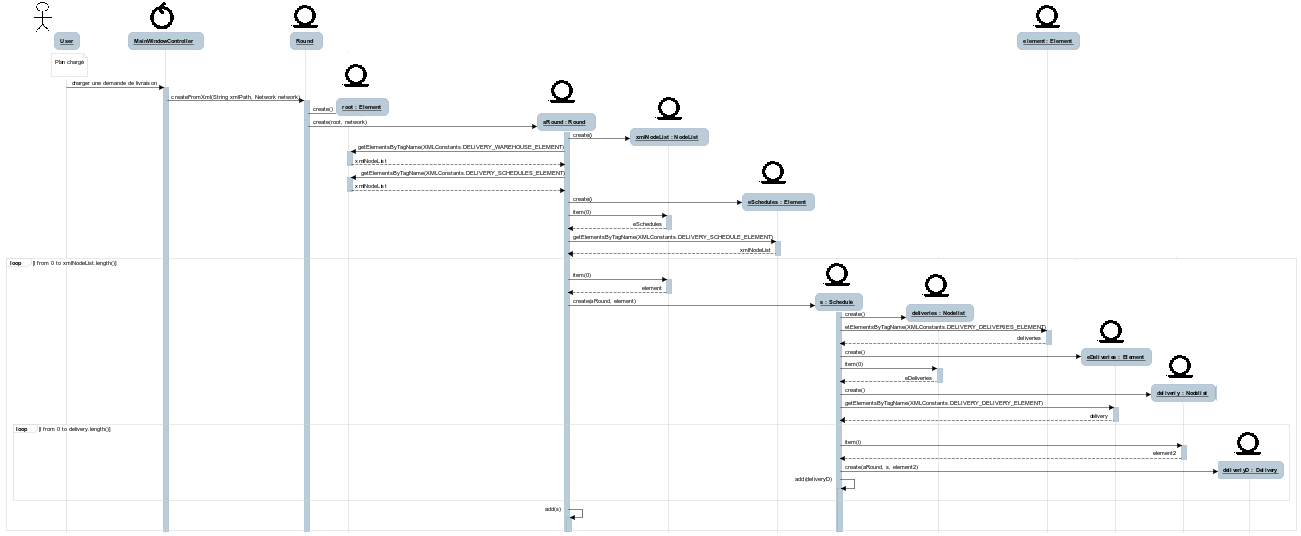
\includegraphics[width=240mm]{../diagrams/sequences/loadRound.png}
        \caption{Diagramme de sequence du chargement de la tourn\'ee}
        \label{diagram:seq_load_round}
    \end{figure}
\end{landscape}
\pagebreak

\begin{landscape}
    \subsection{Calcul d'un tourn\'ee}

    \begin{figure}[h]
        \centering
        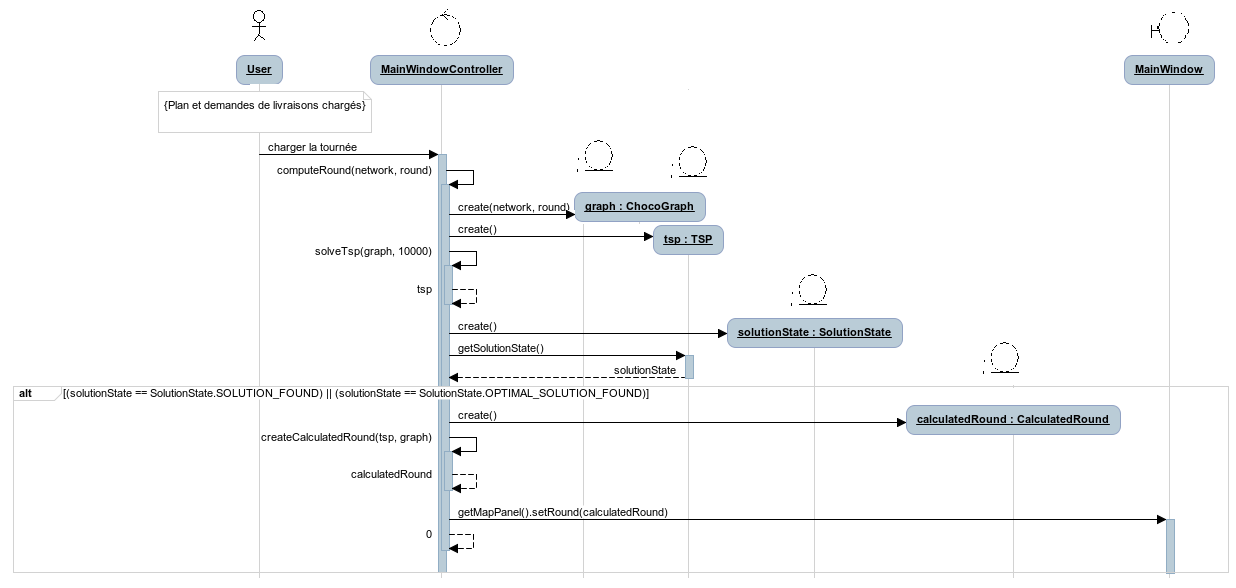
\includegraphics[width=240mm]{../diagrams/sequences/computeRound.png}
        \caption{Diagramme de sequence de calcul de la tourn\'ee}
        \label{diagram:seq_compute_round}
    \end{figure}
\end{landscape}
\pagebreak

\begin{landscape}
    \subsection{Selection d'un noeud de la map}

    \begin{figure}[h]
        \centering
        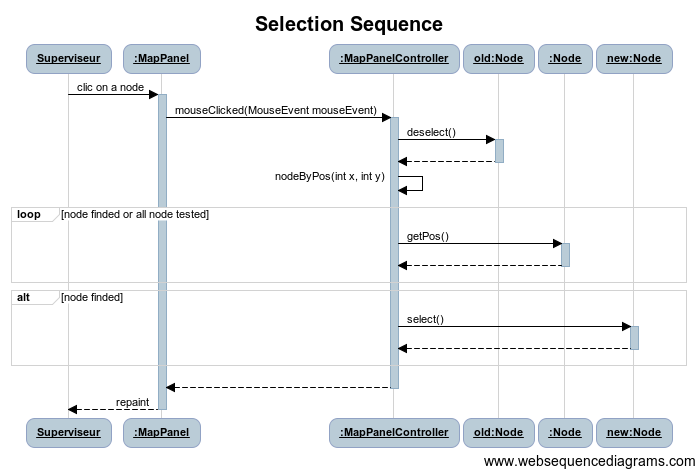
\includegraphics[width=190mm]{../diagrams/sequences/selsequence.png}
        \caption{Diagramme de sequence d'ajout d'une livraison}
        \label{diagram:seq_add_delivery}
    \end{figure}
\end{landscape}
\pagebreak

\begin{landscape}
    \subsection{Ajout d'une livraison}

    \begin{figure}[h]
        \centering
        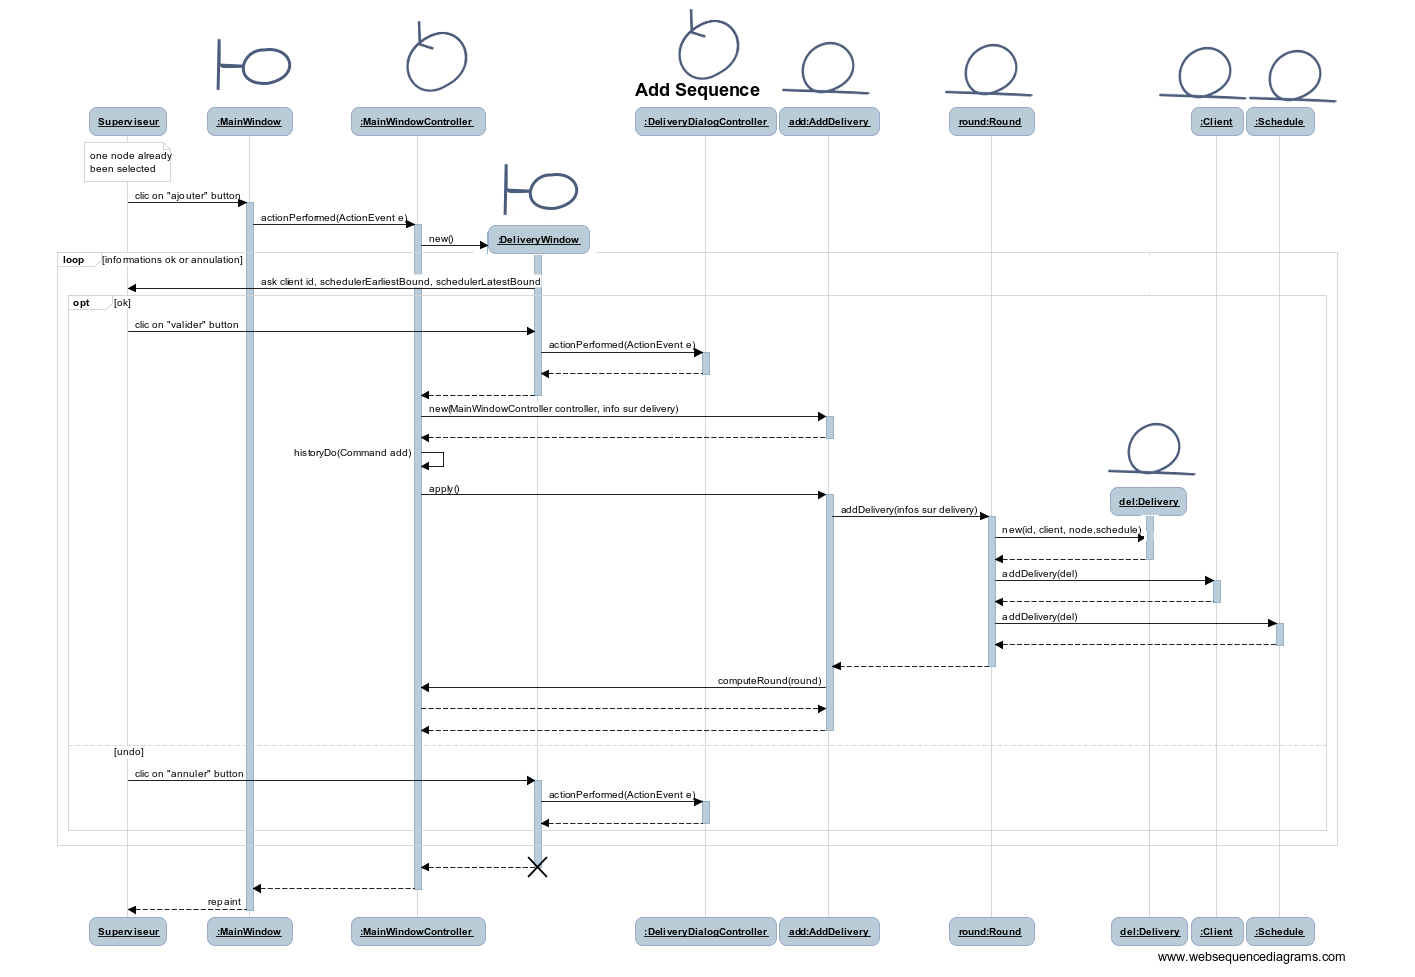
\includegraphics[width=190mm]{../diagrams/sequences/addsequence.png}
        \caption{Diagramme de sequence d'ajout d'une livraison}
        \label{diagram:seq_add_delivery}
    \end{figure}
\end{landscape}
\pagebreak

\begin{landscape}
    \subsection{Suppression d'une livraison}

    \begin{figure}[h]
        \centering
        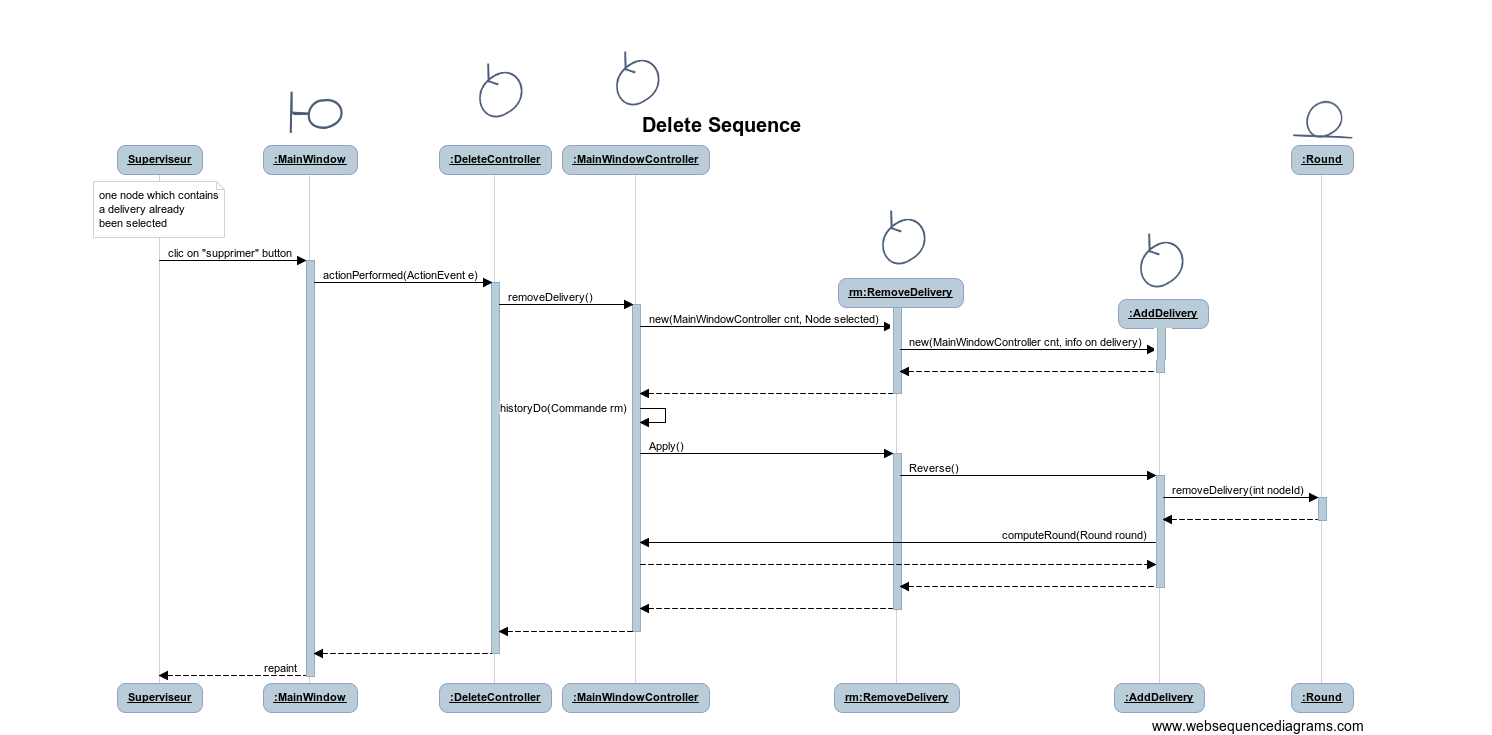
\includegraphics[width=170mm]{../diagrams/sequences/delsequence.png}
        \caption{Diagramme de sequence de suppression d'une livraison}
        \label{diagram:seq_del_delivery}
    \end{figure}
\end{landscape}
\pagebreak
